\section{Il progetto TEPO}
\label{sec:progetto}

\textbf{TEPO} --- \emph{Trento Energy Portfolio Optimizer} --- è un sistema di supporto alla decisione pensato per il Comune di Trento. Il progetto nasce nell'ambito dell'iniziativa ``100 progetti per il Comune di Trento'' ed è sviluppato per il corso di Ingegneria del Software dell'Università degli Studi di Trento (A.A. 2026/2027).

Il problema che ci siamo posti di risolvere non è l'individuazione degli interventi di efficientamento energetico: gli uffici tecnici sanno già quali tipologie sono applicabili ai propri edifici (illuminazione LED, sostituzione dei serramenti, isolamento, pompe di calore, fotovoltaico, caldaie) e dispongono di una stima dei costi e dei benefici attesi. Il problema è un altro, e riguarda il momento della \emph{decisione}: dato un insieme di interventi candidati, un budget limitato e una serie di vincoli tecnici e di policy, quale combinazione conviene finanziare, perché, e come cambierebbe al variare delle risorse disponibili?

\paragraph*{I problemi per l'Amministrazione -}
Le richieste di intervento sono numerose e non è possibile finanziarle tutte. La scelta del portafoglio è un problema combinatorio: con qualche decina di candidati il numero di combinazioni possibili cresce in modo esplosivo e non è affrontabile in modo affidabile con un foglio di calcolo. Le decisioni assunte devono inoltre poter essere ricostruite e giustificate in sede amministrativa, anche a distanza di tempo, e devono essere confrontabili tra loro: due alternative costruite in momenti diversi, o da persone diverse, rischiano di usare criteri e dati non omogenei. Infine, non è quasi mai chiaro quanto una scelta sia ``robusta'': come cambierebbe il portafoglio se il budget aumentasse o diminuisse del 20\%?

\paragraph*{I problemi per gli operatori tecnici -}
I dati di catalogo (edifici, interventi, costi, risparmi, emissioni) sono sparsi tra documenti e fogli di calcolo, con provenienze e formati diversi; non esiste un unico strumento di misura che li renda confrontabili. Gli strumenti automatici disponibili, quando ci sono, tendono a essere opachi: restituiscono una soluzione senza spiegare perché un intervento è stato incluso o escluso, e non lasciano traccia del calcolo. Manca inoltre un modo semplice per confrontare due alternative in modo strutturato, e per verificare se le scelte restano stabili al variare del parametro più discusso in sede politica, cioè il budget.

\paragraph*{La nostra soluzione -}
Il nostro progetto consiste nello sviluppo di \textbf{TEPO}, un'applicazione web che accompagna il Comune attraverso un percorso decisionale esplicito in quattro passi: \emph{configurare} uno scenario, \emph{eseguire} il solver, \emph{confrontare} gli scenari, \emph{verificare la tenuta} delle scelte. TEPO raccoglie in un unico catalogo edifici e opzioni di intervento, con la provenienza del dato sempre visibile; consente di costruire uno scenario scegliendo budget, obiettivo e interventi candidati; calcola con un solver di programmazione matematica il portafoglio ottimo nel rispetto dei vincoli; spiega in modo deterministico, per ogni opzione candidata, perché è stata selezionata o esclusa; permette di salvare due scenari in due slot di confronto (A e B) e di leggerne gli scostamenti; esegue un'analisi di sensibilità sul budget per mostrare cosa resta stabile e cosa oscilla. Un assistente AI \emph{opzionale} può tradurre una richiesta in linguaggio naturale in una proposta di parametri, ma non applica nulla senza un atto esplicito dell'utente.

Il principio architetturale che riassume il progetto è: \textbf{l'AI propone, l'utente confronta, il Comune decide}. TEPO non progetta interventi, non stima costi o benefici, non prende decisioni amministrative: organizza i candidati, valida gli scenari, applica i vincoli, ottimizza, confronta e spiega. La responsabilità della scelta resta in capo alla persona e all'amministrazione.

\subsection*{Gli utenti e il contesto d'uso}
I destinatari principali sono due. L'\textbf{operatore tecnico} del Comune costruisce gli scenari, esegue le ottimizzazioni e analizza i risultati e le motivazioni; è l'utente che interagisce con tutte le funzionalità del sistema. Il \textbf{decisore comunale} (amministratore, dirigente o funzionario) consulta i risultati, le spiegazioni e i confronti per orientare la decisione finale; nell'attuale prototipo il suo ruolo coincide con quello dell'operatore tecnico, ma i contenuti sono progettati per essere letti e condivisi anche da chi non ha partecipato alla configurazione.

Il contesto d'uso è quello di un ufficio tecnico comunale: sessioni di lavoro in ufficio, riunioni tecniche e presentazioni alla cittadinanza. Per questo l'interfaccia prevede due registri di lettura dello stesso strumento --- \emph{Relazione}, pensato per la lettura diurna, la proiezione e la stampa, e \emph{Sala operativa}, pensato per sessioni prolungate di analisi su schermo --- ed è progettata per essere accessibile e stampabile.

\subsection*{I vantaggi}
\begin{itemize}[leftmargin=1.4em, itemsep=0.25em]
    \item \textbf{Rigore e rapidità.} Il portafoglio proposto è la soluzione di un modello matematico, non il risultato di una euristica o di una regola empirica: il sistema espone lo stato del calcolo, se l'ottimalità è stata provata e quali criteri di spareggio sono stati applicati.
    \item \textbf{Riproducibilità e auditabilità.} A parità di scenario il sistema produce sempre lo stesso portafoglio, indipendentemente dall'ordine con cui i candidati sono presentati; ogni esecuzione è registrata con un hash canonico del problema, che permette di ricostruire il calcolo.
    \item \textbf{Trasparenza delle scelte.} Ogni opzione candidata riceve una motivazione deterministica e classificata; la provenienza dei dati (reale, sintetica o mista) e la natura demo del dataset sono dichiarate in modo esplicito e continuativo nell'interfaccia.
    \item \textbf{Confronto e what-if.} Due scenari salvati in A e B si leggono con scostamenti omogenei su investimento, risparmio energetico, risparmio economico, CO\textsubscript{2} e numero di interventi; un'analisi di sensibilità mostra quali selezioni restano stabili al variare del budget.
    \item \textbf{Fiducia nell'automazione.} L'assistente AI è confinato alla proposta di parametri: non calcola risultati, non scrive dati e non applica modifiche senza approvazione umana esplicita. L'applicazione funziona completamente anche in assenza di un modello linguistico esterno.
    \item \textbf{Accessibilità e comunicabilità.} L'interfaccia è progettata per rispettare le linee guida WCAG 2.1 AA, funziona da 320 a 1920 pixel di larghezza, offre due registri visivi e consente di stampare una relazione tecnica del risultato.
\end{itemize}

\subsection*{Le slide del pitch}
Le slide seguenti riproducono le slide informative della presentazione utilizzata durante il pitch: sintetizzano il problema, la soluzione proposta e i benefici attesi. I limiti dell'applicazione, che non hanno una slide dedicata nel pitch, sono illustrati nel testo seguente e ripresi nei requisiti non funzionali.

\begin{figure}[H]
    \centering
    \begin{subfigure}[t]{0.78\linewidth}
        \centering
        
\includegraphics[width=\linewidth]{img/pitch-01-copertina.jpg}
        \caption{Copertina del pitch}
        \label{fig:slide-copertina}
    \end{subfigure}

    \vspace{0.3cm}

    \begin{subfigure}[t]{0.78\linewidth}
        \centering
        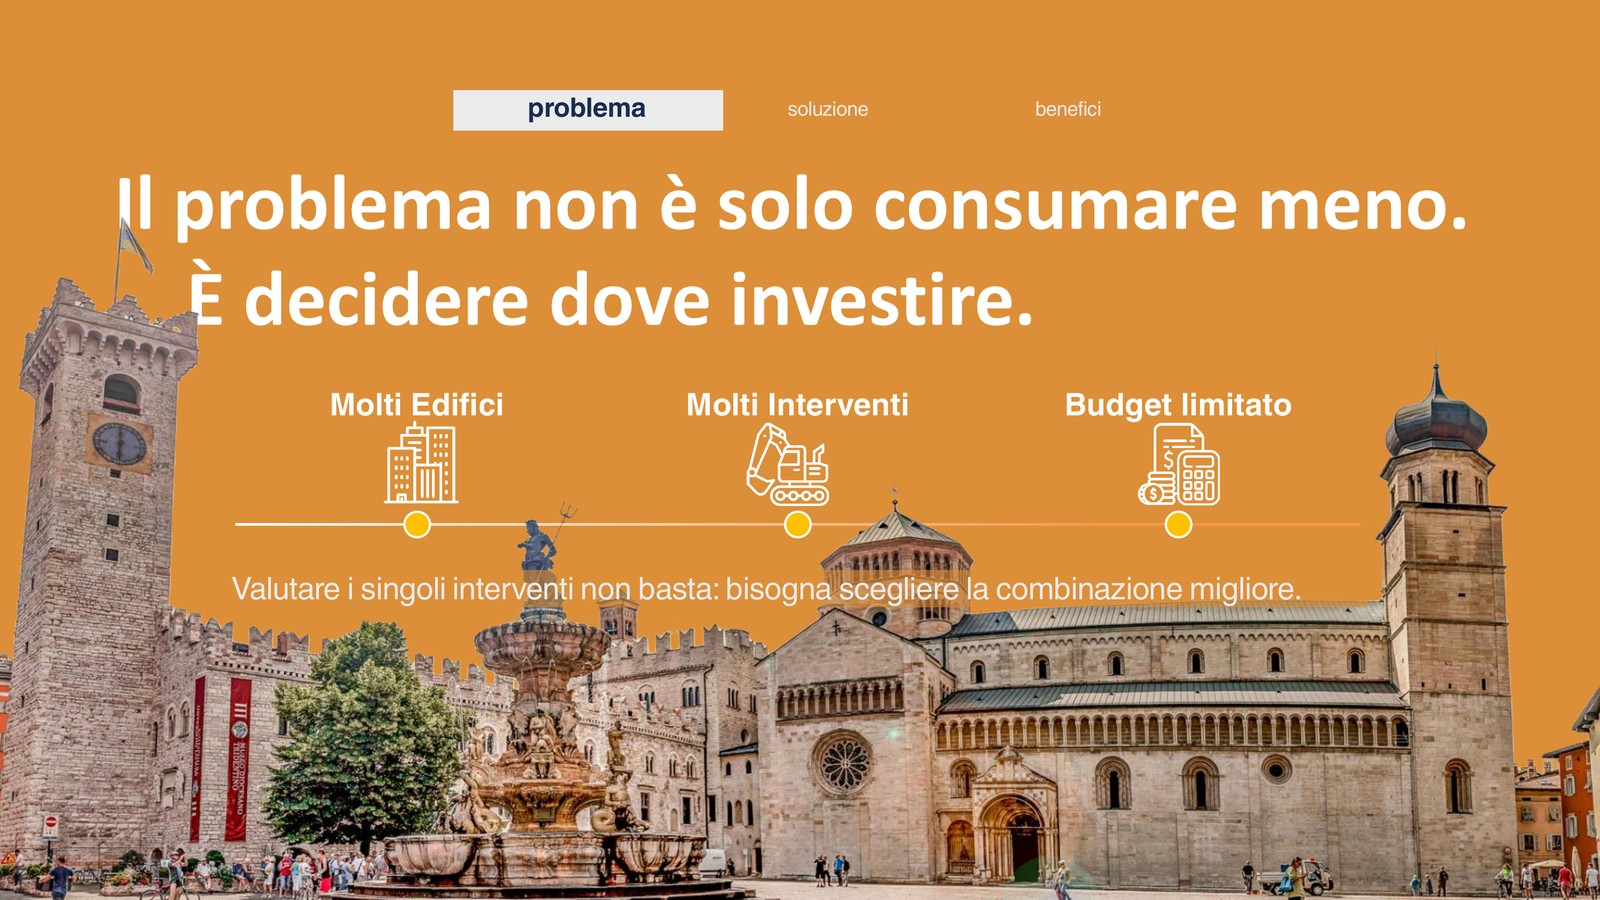
\includegraphics[width=\linewidth]{img/pitch-02-problema.jpg}
        \caption{Il problema: non consumare meno, ma decidere dove investire}
        \label{fig:slide-problema}
    \end{subfigure}
    \caption{Slide del pitch: copertina e problema (prima parte).}
    \label{fig:slides-pitch-1}
\end{figure}

\begin{figure}[H]
    \centering
    \begin{subfigure}[t]{0.78\linewidth}
        \centering
        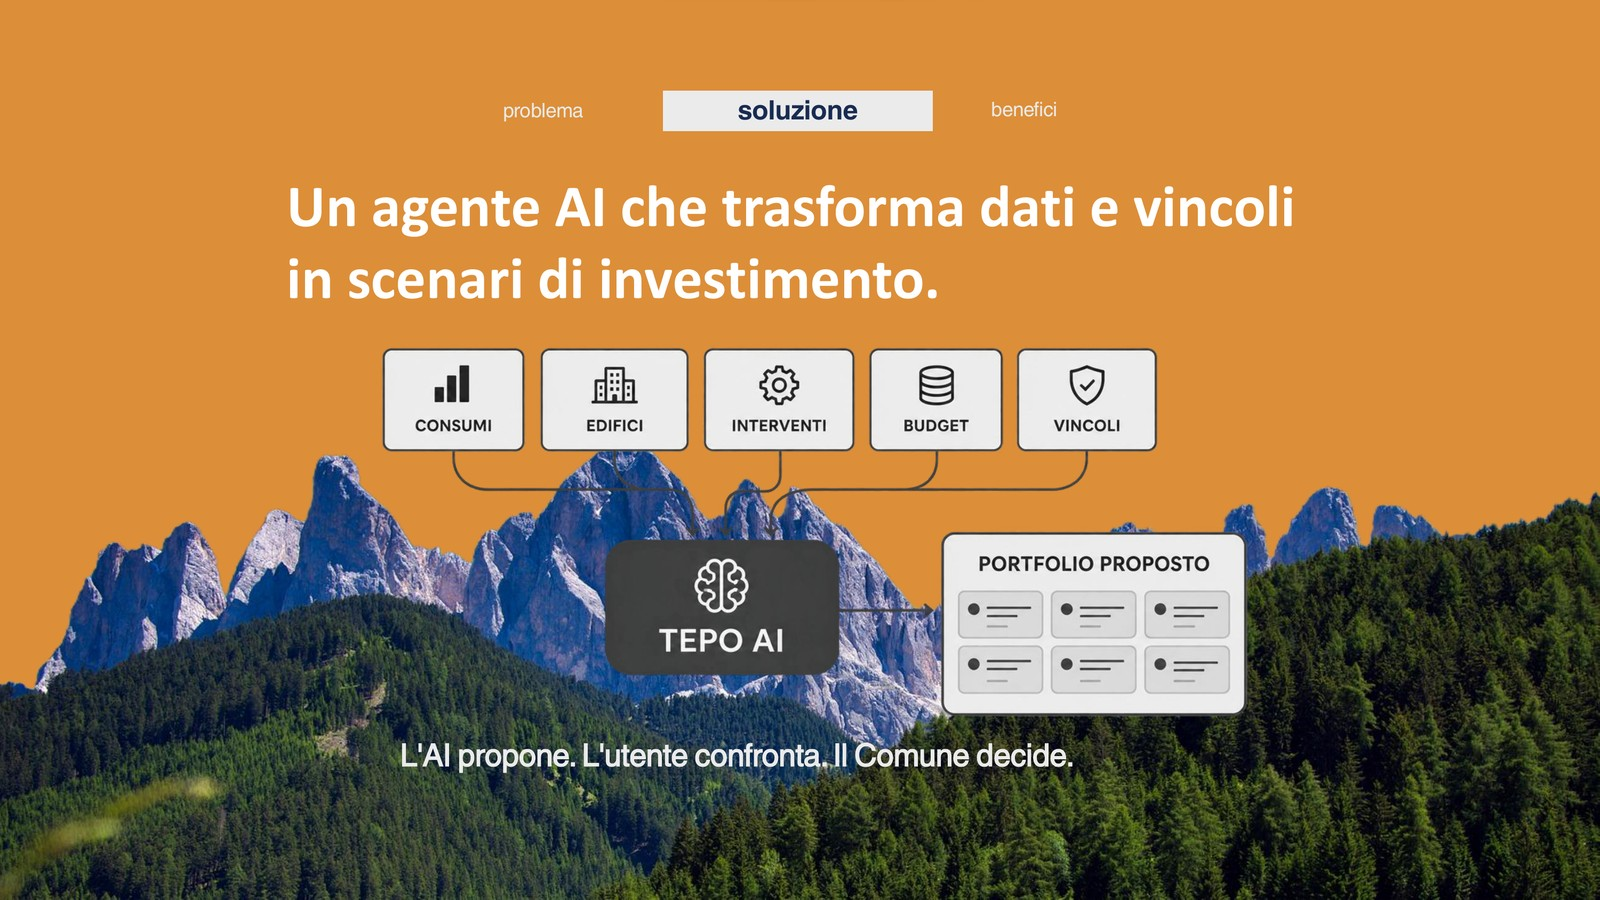
\includegraphics[width=\linewidth]{img/pitch-03-soluzione.jpg}
        \caption{La soluzione: l'agente che trasforma dati e vincoli in scenari}
        \label{fig:slide-soluzione}
    \end{subfigure}

    \vspace{0.3cm}

    \begin{subfigure}[t]{0.78\linewidth}
        \centering
        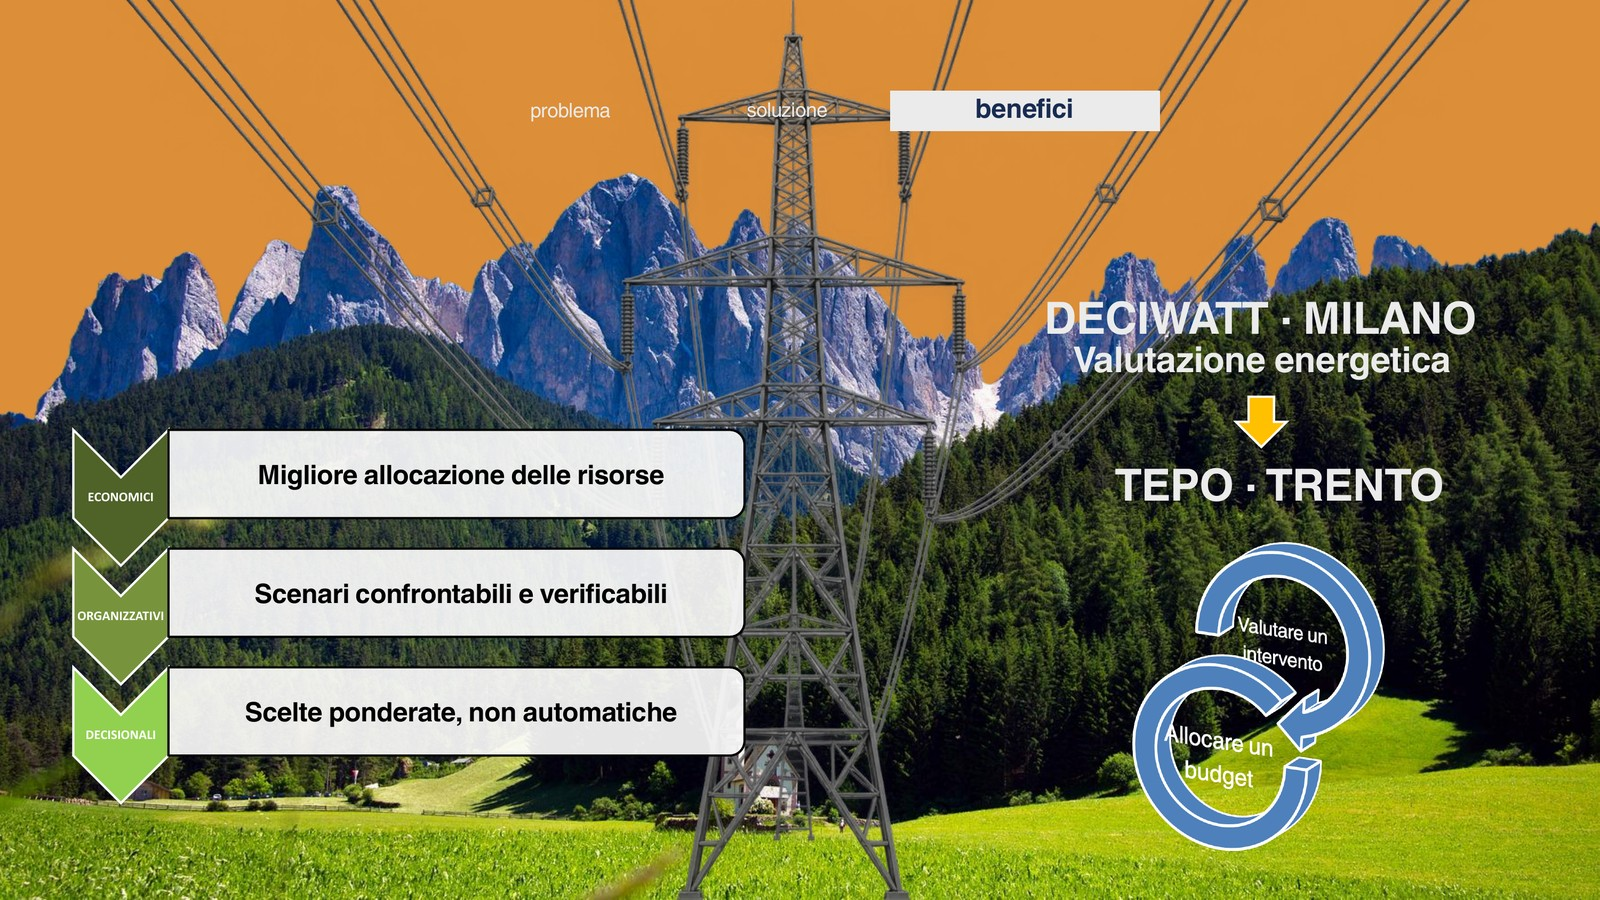
\includegraphics[width=\linewidth]{img/pitch-04-benefici.jpg}
        \caption{I benefici: economici, organizzativi e decisionali}
        \label{fig:slide-benefici}
    \end{subfigure}
    \caption{Slide del pitch: soluzione e benefici (seconda parte).}
    \label{fig:slides-pitch-2}
\end{figure}

\begin{center}
    
\includegraphics[width=0.42\linewidth]{img/pitch-05-chiusura.jpg}\\[0.15cm]
    {\small Slide di chiusura della presentazione.}
\end{center}

\subsection*{I limiti dell'applicazione}
I limiti che seguono sono dichiarati fin dalla baseline e sono parte integrante del progetto: servono a delimitare l'ambito del prototipo e a evitare che i risultati vengano letti come misure ufficiali o come previsioni.

\paragraph{Dataset sintetico e assenza di integrazione}
TEPO lavora su un dataset \textbf{DEMO} interamente sintetico (100 edifici, 300 opzioni di intervento, sei tipologie), costruito per dimostrare il funzionamento del metodo e non per stimare il territorio. Non esiste alcuna integrazione con i sistemi del Comune (catasto, anagrafe, contabilità, portali open data) e nessun dato reale è incluso nell'applicazione. I valori di costo, risparmio e CO\textsubscript{2} sono plausibili ma fittizi; anche il payback mostrato è una stima demo e non una misura ufficiale.

\paragraph{Modello mono-obiettivo}
Il solver ottimizza un obiettivo per volta tra risparmio energetico, risparmio economico e riduzione di CO\textsubscript{2}. Non esiste una combinazione pesata dei tre criteri e non è implementata una frontiera di Pareto: il sistema non propone l'insieme dei portafogli non dominati, ma una sola soluzione per lo scenario scelto. Il confronto A/B e l'analisi di sensibilità aiutano a esplorare il trade-off, ma non lo sostituiscono.

\paragraph{Orizzonte temporale singolo}
Il modello considera un solo periodo: non gestisce la pianificazione multi-anno, lo scaglionamento degli interventi nel tempo, la disponibilità di incentivi negli anni successivi né il monitoraggio dei risultati dopo la realizzazione. Queste funzionalità sono fuori dall'ambito del prototipo e sono elencate come possibili estensioni future.

\paragraph{Spiegazioni locali, non causali}
Le spiegazioni prodotte da TEPO sono deterministiche e verificabili, ma sono \emph{barriere locali}: verificano cosa accadrebbe aggiungendo l'opzione al portafoglio corrente, senza sostituzioni. Non dimostrano che un'opzione non possa entrare in alcun portafoglio ammissibile, e quando la causa dell'esclusione non è deducibile localmente il sistema lo dichiara esplicitamente con la categoria ``causa non determinata''. Inoltre, se esistono più portafogli con lo stesso valore ottimo, il solver ne restituisce uno solo e non segnala l'esistenza di alternative equivalenti.

\paragraph{Assistente AI opzionale e non conversazionale}
L'assistente AI è un supporto alla configurazione, non un decisore: propone parametri a partire da una richiesta in linguaggio naturale, non calcola risultati e non ha accesso in scrittura ai dati. Ogni chiamata è indipendente (non c'è gestione di una conversazione multi-turno) e non esiste alcun addestramento su dati del Comune. Se il provider esterno non è configurato o non risponde, l'applicazione ricade sul motore a regole locale e lo segnala all'utente.

\paragraph{Prototipo, non prodotto}
Il sistema non dispone di autenticazione, gestione dei ruoli o multi-utenza: è pensato per un uso locale di dimostrazione. Gli scenari A/B e l'ultimo risultato sono conservati nella sessione del browser e vengono persi alla chiusura della scheda; il tema scelto, invece, è memorizzato in modo persistente. La configurazione attuale non è pensata per un esercizio reale in produzione.

\paragraph{Prestazioni e scalabilità limitate al dataset di riferimento}
Le prestazioni dichiarate nei requisiti non funzionali sono riferite allo scenario canonico del prototipo e al dataset demo. Non è stato eseguito un collaudo di carico su cataloghi molto più grandi o su più utenti concorrenti, e l'analisi di sensibilità esegue una sequenza di ottimizzazioni indipendenti: all'aumentare dei punti e dei candidati i tempi di risposta crescono.

\paragraph{Non sostituisce il giudizio tecnico e amministrativo}
TEPO non calcola incentivi, tariffe o prezzi reali dell'energia, non verifica la fattibilità tecnica degli interventi e non assume responsabilità decisionali. Il risultato del solver è un supporto alla discussione: la decisione finale resta in capo all'amministrazione e va motivata con gli strumenti ordinari del procedimento amministrativo.
